In order to resolve the shortcomings of existing API governance models in the
cloud, we propose EAGER, a new model and an architecture that can be built
into the cloud fabrics for providing API governance as a cloud-native feature.
EAGER leverages existing SOA governance techniques and 
best practices and adapts them to make them
suitable for cloud platform-level integration.
%have served the SOA community well over the last decade. 
In this section, we
overview the high-level design of EAGER and provide details on its main
components and the policy language.

EAGER is designed to be integrated with extant cloud platforms, 
especially those providing PaaS services. 
It intercepts all events related to application deployment within the cloud
and enforces deployment time governance checks and
logging. 
These governance features include API metadata validation, 
dependency validation, policy validation and 
API backward compatibility
checking. When a policy verification check fails, 
EAGER aborts the deployment of the application and logs the information
necessary to perform remediation.  The goal of EAGER is to maintain the cloud
in a ``governed'' state at all times.  That is, with EAGER active, the cloud
is
automatically prevented from transitioning out of policy compliance due to a
change in the APIs it hosts.

In this work we focus on the deployment-time governance capabilities of EAGER. 
At present, it also implements the same runtime governance features that are
common to most API management facilities (which is necessary but not the
subject of the research we present in this paper).
However, our experience with the interplay between the new deployment-time
governance techniques we discuss and the extant methodologies for runtime
features leads to new possibilities for run time governance as well (which we
discuss as future work).
%providing enforced run-time API governance. We will describe some of these features in this paper, but the final design and implementation of
%run-time API governance is left as future work.

\begin{figure}
\centering
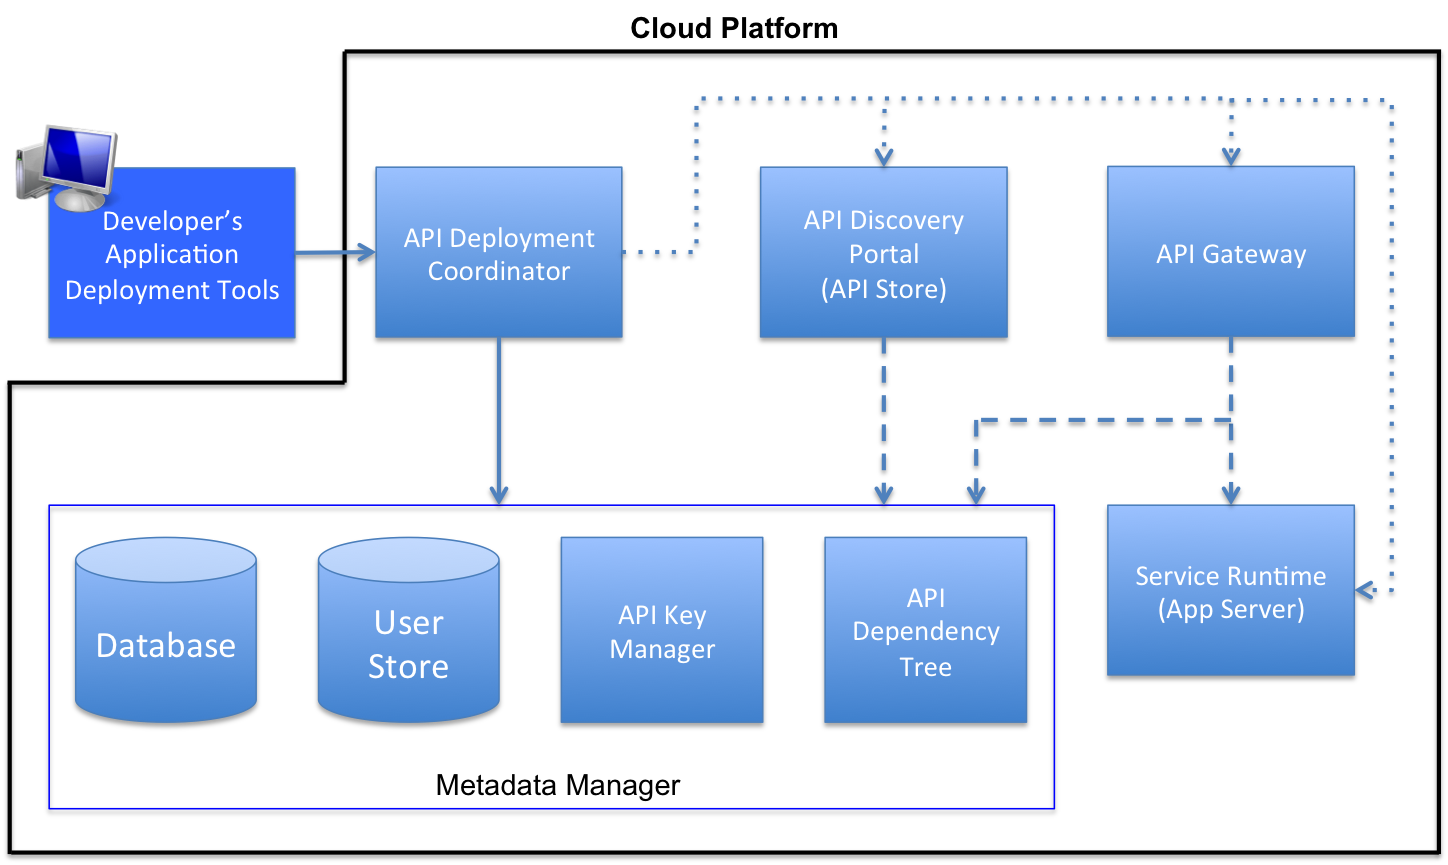
\includegraphics[scale=0.35]{eager_design}
\caption{EAGER Architecture}
\label{fig:eager_design}
\end{figure}

Figure~\ref{fig:eager_design} illustrates the main components of EAGER and
their interactions. Solid arrows represent the interactions that take place
during application deployment time, before an application has been validated
for deployment. Short-dashed arrows indicate the interactions that take place
during deployment time, after an application has been successfully validated.
Long-dashed arrows indicate interactions at run-time.

EAGER is invoked whenever a developer attempts to deploy an application, using
the developer tools available on his/her workstation that activate the target
clouds deployment mechanisms. In some cloud
implementations these tools could be available as an online service accessed
via a web browser. In either case, the application deployment request is
intercepted by the EAGER, which then performs the required governance checks.
If a governance check fails, EAGER will preempt the application deployment,
log relevant data pertaining to the event for later analysis,  and
return an error. Otherwise it proceeds with the application deployment by
activating the deployment mechanisms on the developer's or administrator's
behalf.

The proposed architecture typically does not require major changes to the 
existing components of the cloud since its deployment mechanisms are likely to
be web service based.  EAGER does require integration at the service level,
however ({\em e.g.} it must be a trusted service component in a PaaS cloud). 
%All the 
%EAGER components can be easily implemented as feature additions. 
%The only noteworthy change that is required is the mechanism to intercept application deployment requests and act upon them. 
%This can be done without changing the existing components of the cloud.
%Following subsections further describe the design and responsibilities of EAGER components.

\subsection{Metadata Manager}
The Metadata Manager stores all the API metadata in EAGER. This metadata 
includes API names, versions, specifications and dependencies.
It uses the dependency information to compute the dependency tree (including
versioning information)
among 
all deployed APIs and applications. Additionally, the Metadata Manager
also keeps track of developers, their subscriptions to various APIs and the access credentials (API keys) issued to them. For these purposes,
the Metadata Manager must comprise of some database management system. The developer information may be stored in a specialized user
store (e.g. LDAP).

The Metadata Manager is exposed to other components through a well defined web service interface.
This interface allows querying existing API metadata and updating them. In the proposed model, the stored metadata is updated 
occasionally (only when a new application is deployed or when a developer subscribes to a published API). Therefore the Metadata Manager
does not need to support a very high write throughput. This performance
characteristic allows the Metadata Manager to be implemented with strong 
transactional semantics,
which reduces the development overhead of other components that rely on Metadata Manager. Availability can be improved via
simple replication methods.

\subsection{API Deployment Coordinator} 
The API Deployment Coordinator (ADC)
intercepts all application deployment requests and determines whether they are
suitable for deployment, based on a set of policies specified by the cloud
administrators. It receives application deployment requests via a web service
interface.

An application deployment request contains the name of the application,
version number, names and versions of the APIs exported by the application,
detailed API specifications and other API dependencies as declared by the
developer. Application developers only need to specify explicitly the name and
version of the application and the list of dependencies (i.e. APIs consumed by
the application). All other metadata can be computed automatically by
performing introspection on the application source code. In our prototype
implementation of EAGER, we have developed special tools that perform these
metadata calculations, including the automatic generation of API
specifications.

The API specifications used to describe the web APIs should specify the
operations and the schema of their inputs and outputs.  Any standard API
description language can be used for this purpose, as long as it clearly
describes the schema of the requests and responses. For describing REST
interfaces, we can use Web Application Description Language (WADL), Swagger,
RAML or any other language that provides similar functionality. %Our research
%currently focuses on RESTful 
%services only, but our design can also be adapted to govern SOAP services in
%the cloud, in which case Web Services Description Language (WSDL) can be used
%to create API specifications.

When a new deployment request is received, the ADC checks whether the
application declares any API dependencies. If so, it queries the Metadata
Manager to make sure that all the declared dependencies are already available
in the cloud.  Then it inspects the enclosed application metadata to see if
the current application exports any web APIs. If the application exports at
least one API, the ADC makes another call to the Metadata Manager and pulls
any existing metadata related to that API. If the Metadata Manager cannot
locate any data related to the API in question, ADC assumes it to be a brand
new API (i.e. no previous version of that API has been deployed in the cloud),
and proceeds to the next step of the governance check, which is policy
validation. However, if any metadata regarding the API is found, then the ADC
is dealing with an API update. In this case, the ADC compares the old API
specifications with the latest ones provided in the application deployment
request to see if they are compatible.

To perform this API compatibility verification, the ADC checks to see whether
the latest specification of an API contains all the operations available in
the old specification. If the latest API specification is missing at least one
operation that it used to have, the ADC reports this to the user and aborts
the deployment. If all the past operations are present in the latest
specification, the ADC performs a type check to make sure that all past and
present operations are type compatible. This is done by performing recursive
introspection on the input and output types declared in the API
specifications. EAGER looks for type compatibility based on the following
rules inspired by Hoare logic~\cite{Hoare:1969:ABC:363235.363259} and the
rules of type inheritance from object oriented programming:
\begin{itemize}
\item New version of an input type is compatible with the old version of an input type, if the new version contains either all or less attributes than the 
old version, and any new attributes that are unique to the new version are optional.
\item New version of an output type is compatible with the old version of an output type, if the new version contains either all or more attributes than the 
old version.
\end{itemize}
In addition to the type checks, ADC may also compare other parameters declared in the API specifications
such as HTTP methods, mime types and URL patterns.

%There is a significant optimization possible when performing these API specification comparison. In addition to the API specifications,
%the Metadata Manager can report to the ADC, whether the API being validated is already being used by any other application. 
%If no other application is using the API being validated, then EAGER
%can completely skip the API specification comparison phase, since in this case even a backwards incompatible API change will not break any 
%downstream application. 
%Based on how much metadata is available to perform this computation, EAGER can choose to do further optimizations too. For example, if
%the Metadata Manager keeps track of which operations of an API are being used by other applications, we can restrict the specification compatibility
%check to only compare the operations that are in active use, thus greatly narrowing down the scope of the specification validation check.

Once the API specifications have been successfully compared without errors,
the ADC initiates policy validation. Policies are specified by cloud
administrators or administrators of the organization (tenant) that the
application developer is part of. Policies are specified using a subset of the
Python programming language, 
which makes it easy to develop and maintain them.
%We control the built-in Python functions and modules policy files may engage
%via a simple whitelisting method. 
We also define a set of assertions
that policy writers can use to specify various checks that must be performed
on the applications. 
Currently this assertion list includes:
\begin{lstlisting}[language=Python, frame=single]
assert_true(condition, optional_error_msg)
assert_false(condition, optional_error_msg)
assert_app_dependency(app, 
  d_name, d_version)
assert_not_app_dependency(app, 
  d_name, d_version)
assert_app_dependency_in_range(app, name, 
  lower, upper, 
  exclude_lower, exclude_upper)
\end{lstlisting}

%\begin{itemize}
%\item assert\_true(condition, optional\_error\_msg)
%\item assert\_false(condition, optional\_error\_msg)
%\item assert\_app\_dependency(app, d\_name, d\_version)
%\item assert\_not\_app\_dependency(app, d\_name, d\_version)
%\item assert\_app\_dependency\_in\_range(app, name, lower, upper, exclude\_lower, exclude\_upper)
%\end{itemize}

%Using the above assertions and the restricted Python syntax it is possible to
%implement even the most complex policies in a simple and intuitive manner.
Basing the policy language on Python allows EAGER to leverage
%Using a real programming language for specifying policies naturally lends
%itself to using 
existing programming tools to edit and debug policy files. An example policy
file that mandates all application names to begin with upper case letters and,
all applications to take a dependency on an API called Logger-v1.0 is shown
below:

\begin{lstlisting}[language=Python, frame=single]
import re

pattern = re.compile(`^[A-Z]')
assert_true(pattern.match(app.name))
assert_app_dependency(app,`Logger',`1.0')
\end{lstlisting}

In the above example \textit{app} is a special logical variable available to
all policy files. This variable allows applications to access information
pertaining to the current application deployment request. 

EAGER has no restrictions on how many policy files can be specified by the
administrators. Applications are validated against each policy file. Failure
of any assertion in any policy file will cause the ADC to abort the
application deployment. Once an application has been checked against all
applicable policies, ADC persists the latest application and API metadata into
the Metadata Manager.  At this point, the ADC may report success to the user
and proceed with rest of the application deployment. In a PaaS setting
this deployment
activity typically involves three
steps:

\begin{enumerate}
\item Deploy the application in the cloud application runtime (application server).
\item Publish the APIs enclosed in the application and their specifications to
API Discovery Portal or catalog.
\item Publish the APIs enclosed in the application to an API Gateway server.
\end{enumerate}

Step 1 is required to complete the application deployment in the cloud even without EAGER. The significance of steps 2 and 3 is explained in the 
following subsections.

\subsection{API Discovery Portal} API Discovery Portal (ADP) is an online
catalog, where developers can browse the available web APIs. Whenever the ADC
approves and deploys a new application, it registers all the APIs exported by
the application in ADP.  EAGER mandates that any developer interested in using
an API, first subscribe to that API and obtain the proper credentials (API
keys) from the ADP. The API keys issued by the ADP could be an
OAuth~\cite{oauth2} access
token (as is typically of many REST-based web services) 
or a similar authorization credential, that can be used to verify the
developer/application that is invoking the API. This credential management
function is
important both to auditing and also as a connection to
runtime governance since it gives EAGER the ability to identify
the developers/applications that are using the APIs. 

The API keys issued by the ADP are stored in the Metadata Manager. When a
programmer develops a new application using one or more API dependencies, we
may mandate that the developer declares the dependencies along with the API
keys obtained from the ADP. The ADC can then verify this information against
the Metadata Manager as a part of its dependency check, and ensure that the
declared dependencies are correct and the specified API keys are valid. 

Deployment-time governance policies
may further incentivize the declaration of API 
dependencies explicitly by making it 
impossible to call an API without first declaring it as a dependency along
with the proper API keys. These types of policies can be implemented
by making some changes to the
application runtime in the cloud, so that it loads the API credentials from
the dependency declaration provided by the application developer.
%  Currently
%neither EAGER nor any of the extant runtime governance facilities provide this
%linkage between deployment and runtime governance.

\subsection{API Gateway} 
Runtime governance of applications by systems such as
Synapse~\cite{synapse} make use of an API ``proxy'' or gateway.
%API Gateway is another piece of the runtime
%governance puzzle that we intend to solve as a part of our future work. 
It
intercepts all API calls and validates the API keys provided in them. The
traffic interception is achieved by blocking direct access to the APIs in the
application runtime (app servers), and publishing the API Gateway address as
the API endpoint in the ADP. The first can be achieved via a simple firewall
or router configuration that prevents the cloud app servers from receiving any
API traffic from a source other than the API Gateway. Once an API call has
been received and validated at the API Gateway, the message is routed to the
actual application server in the cloud that hosts the API.

The API Gateway can be a single server or a cluster of servers 
behind a scalable load balancer. %Since most API metadata, especially the API keys, do not change
%frequently, it can afford to cache such information locally for better runtime performance. 
In addition to API key validation, it may perform other
functions as well, such as monitoring, throttling (rate limiting), SLA
enforcement and runtime policy validation. We intend to further evaluate these
runtime governance features and they way the must be integrated with
EAGER deployment-time governance
in our future research.
